\section{Jatkotutkimusaiheita}

Luvussa \ref{tulokset} selvisi, että pistedatan kompressoiminen johtaa pienempien tiedostokokojen lisäksi myös oktettipuun rakentamisen nopeutumiseen. Toisaalta kompression purkaminen vie runsaasti laskenta-aikaa renderöintivaiheessa. Laitossuunnitteluohjelmistossa tallennustilan tehokas käyttö ja pistepilven saaminen nopeasti katsottavaksi ovat tärkeää, joten olisi syytä tutkia, saadaanko kompression purkamista nopeutettua. Yksi mahdollisuus olisi säikeistää pisteiden lataamista niin, että yksi säie lukee pisteitä levyltä, toinen purkaa niiden kompressiota ja kolmas kopioi niitä näytönohjaimelle.

Oktettipuun solmujen järjestäminen ruudulle projisoidun koon mukaan vei runsaasti laskenta-aikaa, minkä johdosta luvussa \ref{render} esitetty renderöintialgoritmi suoriutui heikosti suoraviivaiseen puskurivirralla renderöintiin verrattuna. Voidaan kuitenkin katsoa renderöidyn pistepilven korkeamman tiheyden kameran lähellä olevan tärkeämpää kuin absoluuttinen pisteiden määrä. Solmujen järjestämistä voisi myös nopeuttaa helposti säikeistämällä renderöintialgortimi niin, että yksi säie valikoi puusta solmuja prioriteettijonoon, josta toinen säie ottaa aina suurimman prioriteetin omaavan solmun renderöitäväksi.

Pistebudjetin käyttö pistepilveä renderöitäessä mahdollistaa interaktiivisen ruudunpäivitysnopeuden, mutta huonontaa renderöidyn kuvan laatua. Kuvassa \ref{lod_border} näkyy ilmanvaihtohuoneen katossa ikäviä tarkkuustasojen eroja. Kun puusta renderöidään solmuja niiden kuvaruudulle projisoidun koon mukaan eikä taso kerrallaan, voi kuvassa esiintyä suuria tiheyseroja. Tiheyseroja voisi vähentää ja kuvan laatua parantaa implementoimalla esimerkiksi Schützin \cite{potree} ehdottaman muokkautuvan pistekoon algoritmin. 

\begin{figure}
    \centering
    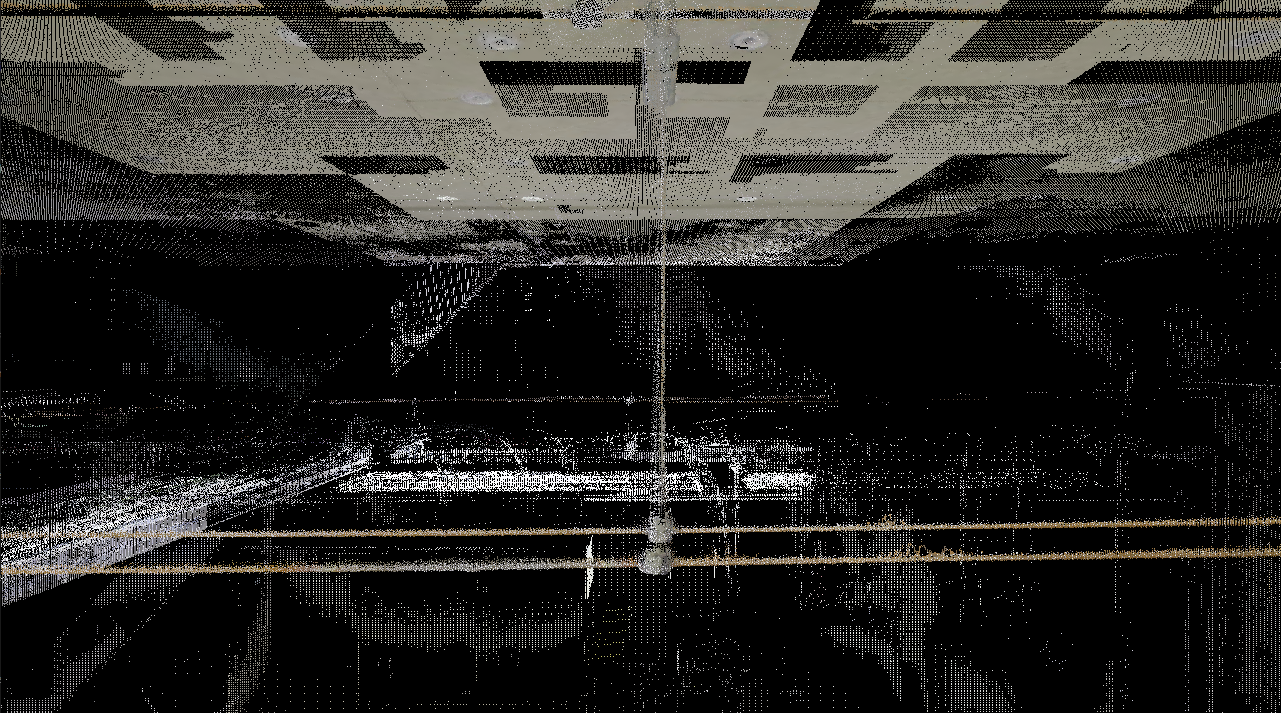
\includegraphics[width=0.7\textwidth]{tuloksia/ilmastointi_2M/ilmastointihuone_vesijohto_overviewbuf.png}
    \caption{Kahden miljoonan pisteen budjetin käyttäminen aiheuttaa ilmanvaihtohuone-pilvessä häiritseviä tarkkuustasojen välisiä eroja.}
    \label{lod_border}
\end{figure} 